% Auto-generated by experiments/plot_scaled_derivative_families.py.
% Requires \usepackage{pgfplots} and \pgfplotsset{compat=1.18}.
% Figure label suggestion: \label{fig:scaled-exit-surface}
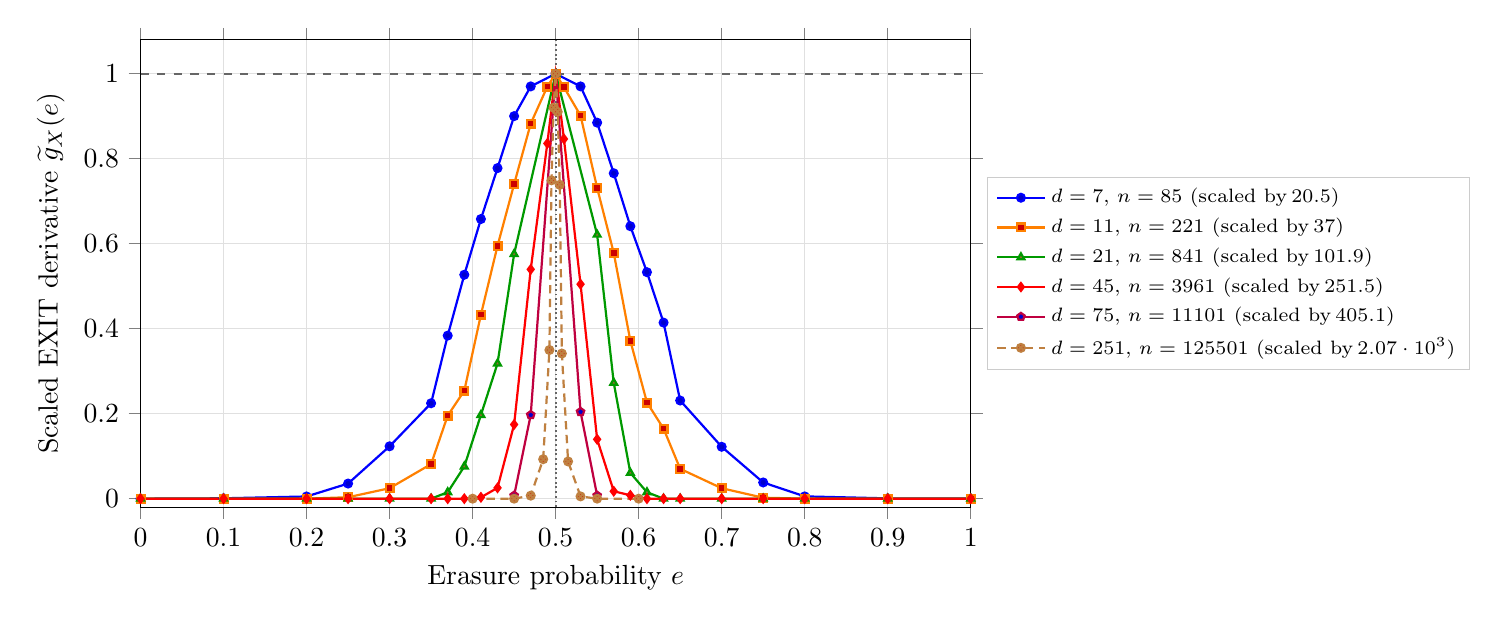
\begin{tikzpicture}
\begin{axis}[
  name=scaledEXITSurfaceAxis,
  width=\linewidth,
  height=0.62\linewidth,
  xlabel={Erasure probability $e$},
  ylabel={Scaled EXIT derivative $\widetilde g_X(e)$},
  xmin=0, xmax=1,
  ymin=-0.02, ymax=1.08,
  grid=both,
  major grid style={black!12},
  minor grid style={black!6},
  tick align=outside,
  legend cell align={left},
  legend style={draw=black!20, fill=white, at={(1.02,0.5)}, anchor=west, font=\scriptsize},
]
\addplot[black!60, densely dotted, line width=0.7pt, forget plot] coordinates {(0.5,-0.02) (0.5,1.08)};
\addplot[black!60, dashed, line width=0.7pt, forget plot] coordinates {(0,1) (1,1)};
\addplot+[color=blue, mark=*, mark size=1.4pt, line width=0.8pt]
coordinates {(0,0) (0.1,0.000884955752212) (0.2,0.00514883346742) (0.25,0.0355591311344) (0.3,0.123250201126) (0.35,0.224571888289) (0.37,0.383748994368) (0.39,0.526950925181) (0.41,0.658085277554) (0.43,0.777956556718) (0.45,0.900241351569) (0.47,0.970233306516) (0.5,1) (0.53,0.970233306516) (0.55,0.884955752212) (0.57,0.765888978278) (0.59,0.641190667739) (0.61,0.532984714401) (0.63,0.414320193081) (0.65,0.231007930123) (0.7,0.122123893805) (0.75,0.0381335478681) (0.8,0.00536336819523) (0.9,0.000724054706356) (1,0.000160901045857)};
\addlegendentry{$d=7$, $n=85$ ($\mathrm{scaled\ by}\,20.5$)}
\addplot+[color=orange, mark=square*, mark size=1.4pt, line width=0.8pt]
coordinates {(0,0) (0.1,0) (0.2,0) (0.25,0.00335195530726) (0.3,0.0245810055866) (0.35,0.0814046288907) (0.37,0.195530726257) (0.39,0.254189944134) (0.41,0.432960893855) (0.43,0.594972067039) (0.45,0.740223463687) (0.47,0.882681564246) (0.49,0.969832402235) (0.5,1) (0.51,0.96834264432) (0.53,0.901675977654) (0.55,0.731284916201) (0.57,0.578212290503) (0.59,0.371508379888) (0.61,0.22625698324) (0.63,0.164804469274) (0.65,0.0702314445331) (0.7,0.0245810055866) (0.75,0.00223463687151) (0.8,0) (0.9,0) (1,0)};
\addlegendentry{$d=11$, $n=221$ ($\mathrm{scaled\ by}\,37$)}
\addplot+[color=green!60!black, mark=triangle*, mark size=1.4pt, line width=0.8pt]
coordinates {(0,0) (0.1,0) (0.2,0) (0.25,0) (0.3,0) (0.35,0) (0.37,0.0151515151515) (0.39,0.0757575757576) (0.41,0.19696969697) (0.43,0.318181818182) (0.45,0.575757575758) (0.5,1) (0.55,0.621212121212) (0.57,0.272727272727) (0.59,0.0606060606061) (0.61,0.0151515151515) (0.63,0) (0.65,0) (0.7,0) (0.75,0) (0.8,0) (0.9,0) (1,0)};
\addlegendentry{$d=21$, $n=841$ ($\mathrm{scaled\ by}\,101.9$)}
\addplot+[color=red, mark=diamond*, mark size=1.4pt, line width=0.8pt]
coordinates {(0,0) (0.1,0) (0.2,0) (0.25,0) (0.3,0) (0.35,0) (0.37,0) (0.39,0) (0.41,0.0031746031746) (0.43,0.0253968253968) (0.45,0.174603174603) (0.47,0.539682539683) (0.49,0.835978835979) (0.5,1) (0.51,0.846560846561) (0.53,0.504761904762) (0.55,0.139682539683) (0.57,0.0174603174603) (0.59,0.00793650793651) (0.61,0) (0.63,0) (0.65,0) (0.7,0) (0.75,0) (0.8,0) (0.9,0) (1,0)};
\addlegendentry{$d=45$, $n=3961$ ($\mathrm{scaled\ by}\,251.5$)}
\addplot+[color=purple, mark=pentagon*, mark size=1.4pt, line width=0.8pt]
coordinates {(0.45,0.00729927007299) (0.47,0.197080291971) (0.5,1) (0.53,0.204379562044) (0.55,0.00729927007299)};
\addlegendentry{$d=75$, $n=11101$ ($\mathrm{scaled\ by}\,405.1$)}
\addplot+[color=brown, mark=otimes*, mark size=1.4pt, line width=0.8pt]
coordinates {(0.4,0) (0.45,0) (0.47,0.00707213578501) (0.485,0.0928492849285) (0.4925,0.349834983498) (0.495,0.749174917492) (0.4975,0.920132013201) (0.5,1) (0.5025,0.910231023102) (0.505,0.738613861386) (0.5075,0.341584158416) (0.515,0.0875687568757) (0.53,0.00537482319661) (0.55,4.71475719e-05) (0.6,0)};
\addlegendentry{$d=251$, $n=125501$ ($\mathrm{scaled\ by}\,2.07\cdot 10^{3}$)}
\end{axis}
\end{tikzpicture}
